\documentclass[12pt,letterpaper]{article}
\usepackage[utf8]{inputenc}
\usepackage[spanish]{babel}
\usepackage{graphicx}
\usepackage[left=2cm,right=2cm,top=2cm,bottom=2cm]{geometry}
\usepackage{graphicx} % figuras
% \usepackage{subfigure} % subfiguras
\usepackage{float} % para usar [H]
\usepackage{amsmath}
%\usepackage{txfonts}
\usepackage{stackrel} 
\usepackage{multirow}
\usepackage{enumerate} % enumerados
\renewcommand{\labelitemi}{$-$}
\renewcommand{\labelitemii}{$\cdot$}
% \author{}
% \title{Caratula}
\begin{document}

% Fancy Header and Footer
% \usepackage{fancyhdr}
% \pagestyle{fancy}
% \cfoot{}
% \rfoot{\thepage}
%

% \usepackage[hidelinks]{hyperref} % CREA HYPERVINCULOS EN INDICE

% \author{}
\title{Caratula}

\begin{titlepage}
\begin{center}
\large{UNIVERSIDAD PRIVADA-DE-TACNA}\\
\vspace*{-0.025in}
\begin{figure}[htb]
\begin{center}

\includegraphics[width=8cm]{./Imagenes/logo}
\end{center}
\end{figure}
\vspace*{0.15in}
INGENIERIA DE SISTEMAS  \\

\vspace*{0.5in}
\begin{large}
TITULO:\\
\end{large}

\vspace*{0.1in}
\begin{Large}
\textbf{LABORATORIO Nro 02} \\
\end{Large}

\vspace*{0.3in}
\begin{Large}
\textbf{CURSO:} \\
\end{Large}

\vspace*{0.1in}
\begin{large}
INTELIGENCIA DE NEGOCIOS\\
\end{large}

\vspace*{0.3in}
\begin{Large}
\textbf{DOCENTE(ING):} \\
\end{Large}
\vspace*{0.1in}
\begin{large}
 Patrick Cuadros Quiroga\\
\end{large}
\vspace*{0.2in}
\vspace*{0.1in}
\begin{large}
Integrantes: \\
\begin{flushleft}


Samuel Nuñez Mamani         	    \hfill	(2016054462) \\


\end{flushleft}
\end{large}
\end{center}

\end{titlepage}


\section{Desarrollo} 
\begin{itemize}

	\item 1. Ejercicio 1 : Las relaciones creadas automáticamente
		\begin{figure}[H]
		\begin{center}
		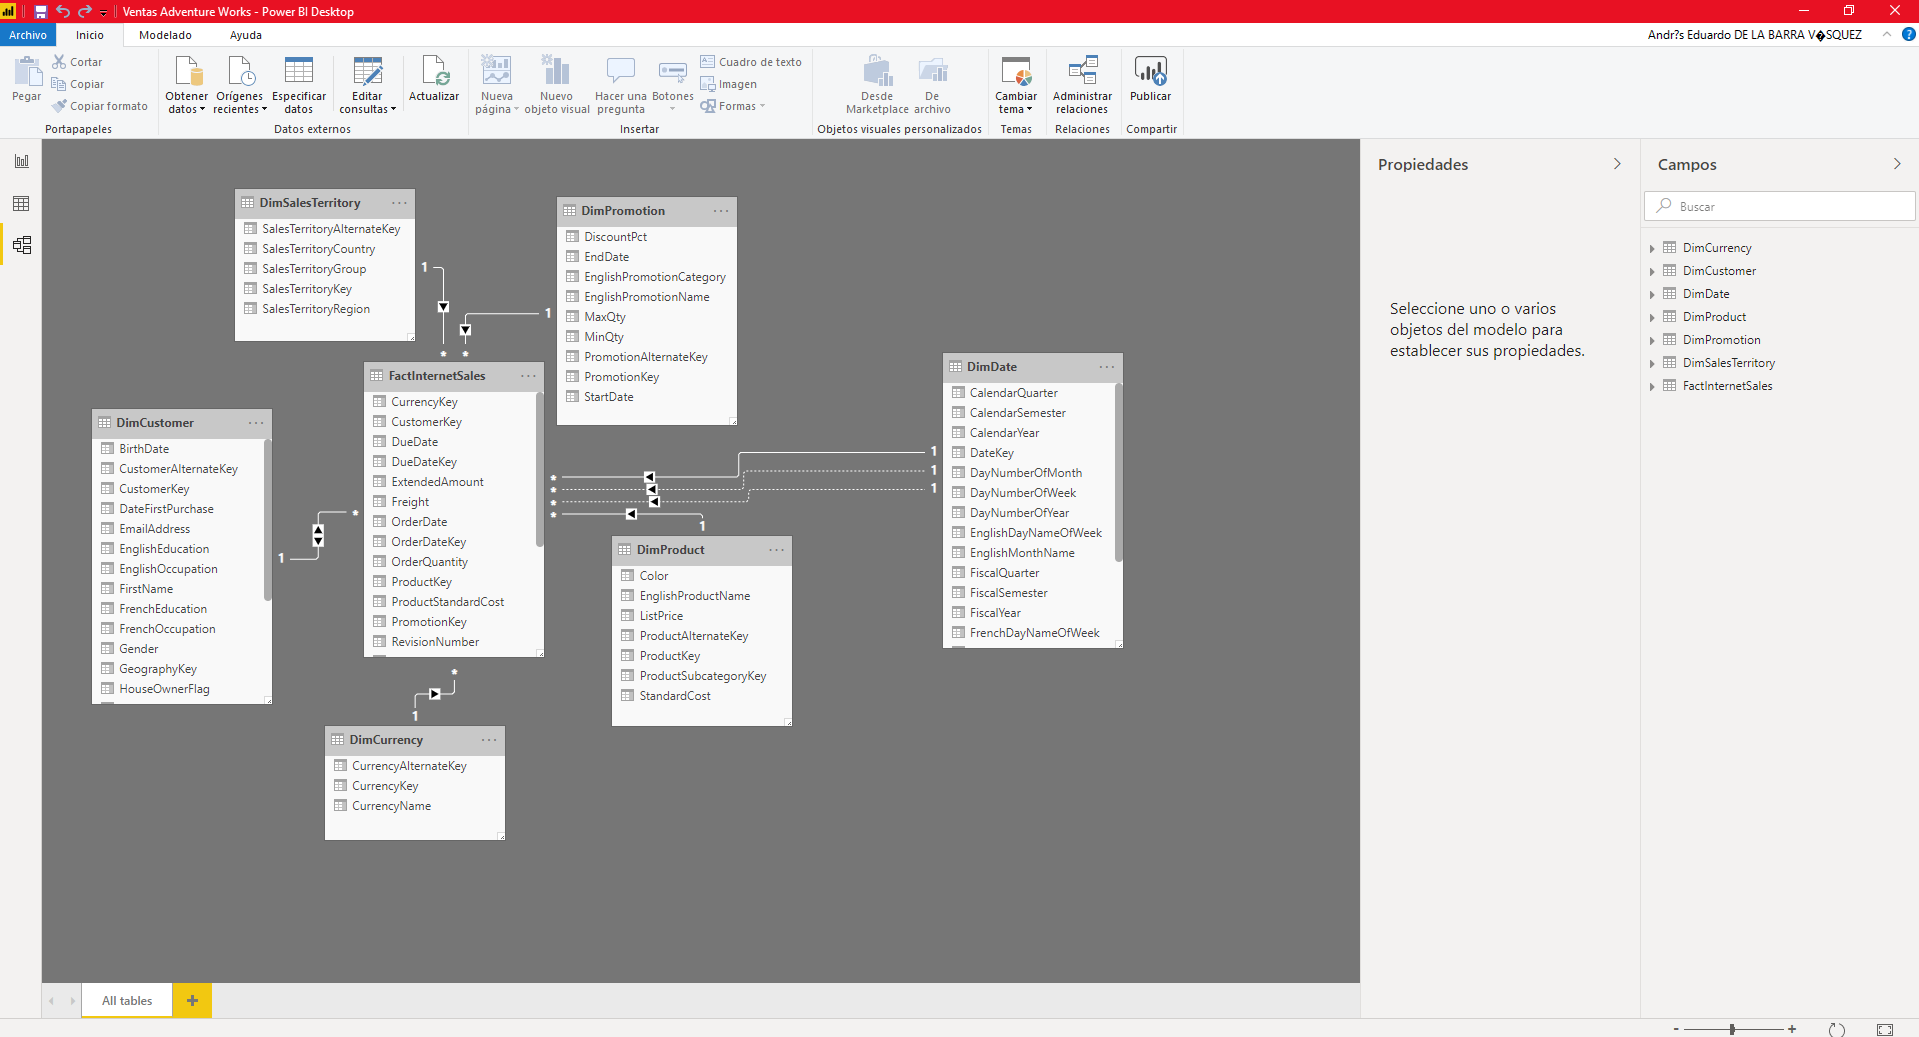
\includegraphics[width=18cm]{./Imagenes/imagen1}
		\end{center}
		\end{figure}

     	\item2. Ejercicio1: Relaciones manuales  
		\begin{figure}[H]
		\begin{center}
		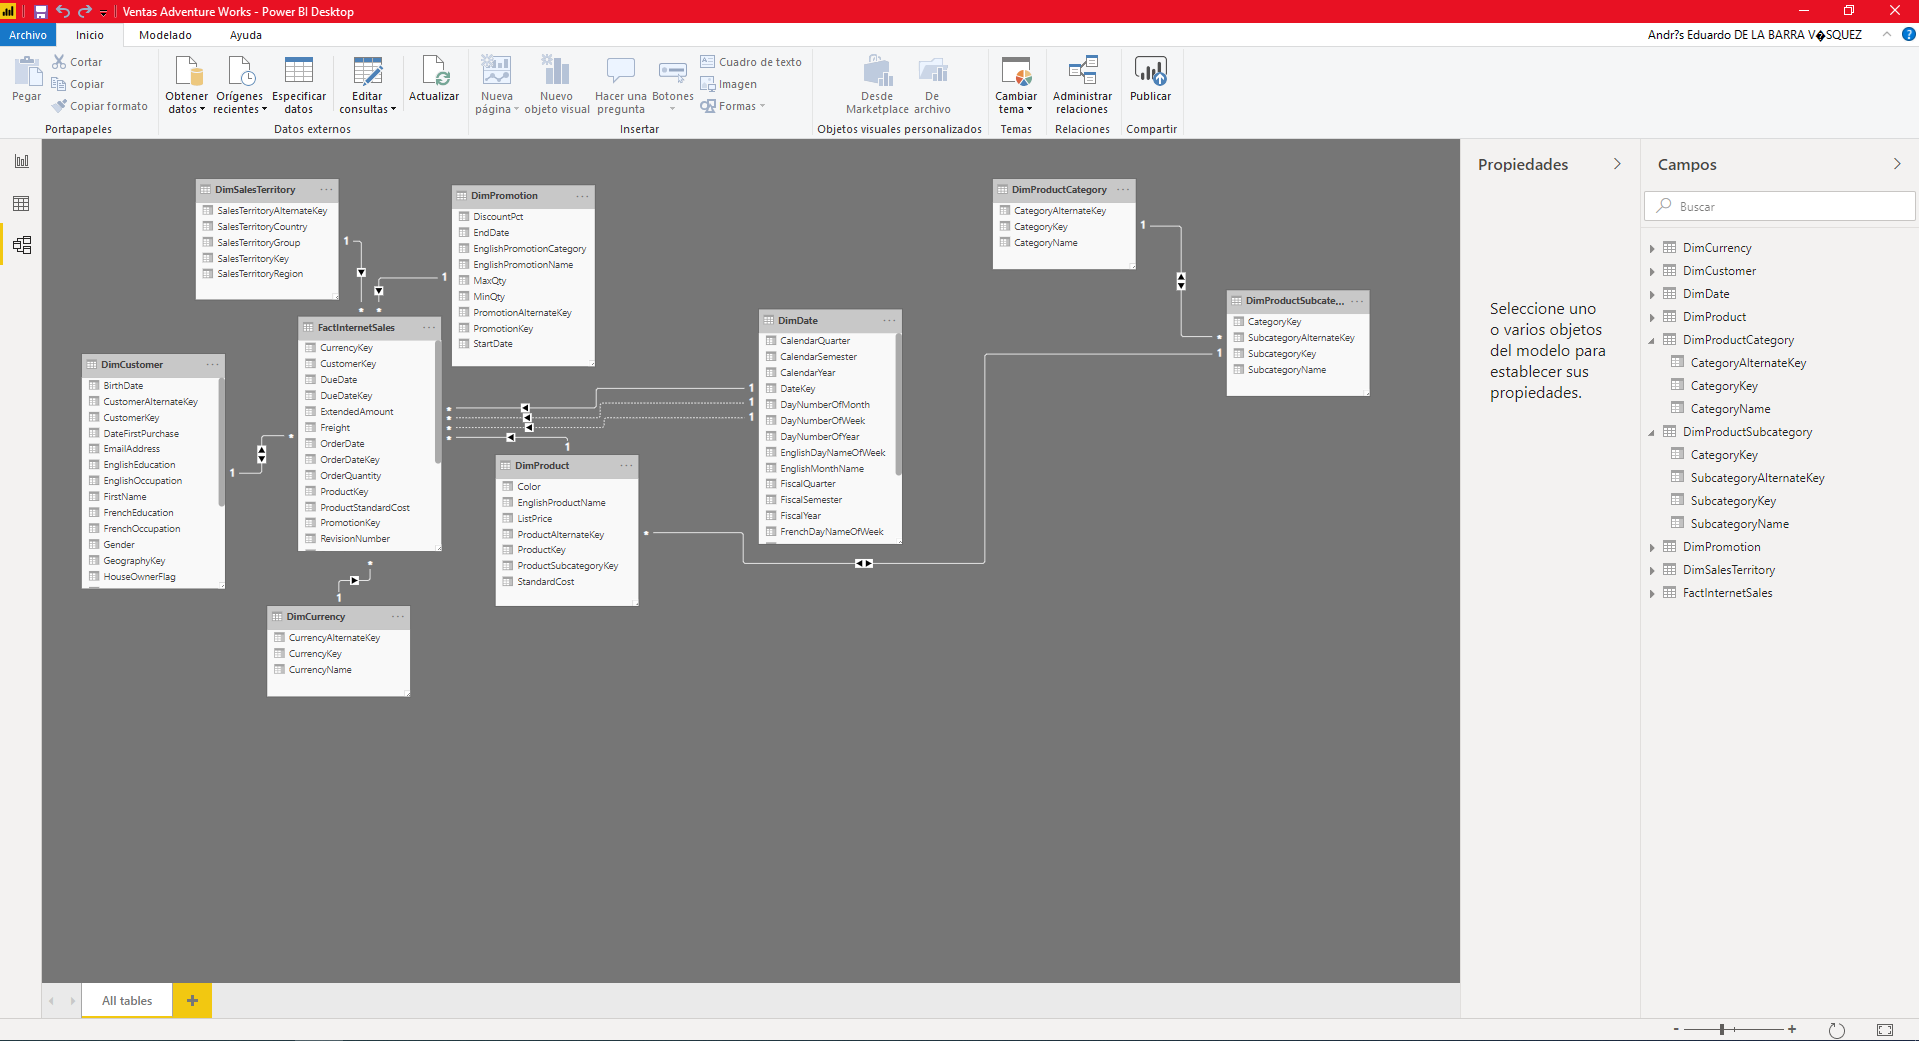
\includegraphics[width=18cm]{./Imagenes/imagen2}
		\end{center}
		\end{figure}
     
	\item3. Ejercicio 2: Query en la tabla DimCustomer
		\begin{figure}[H]
		\begin{center}
		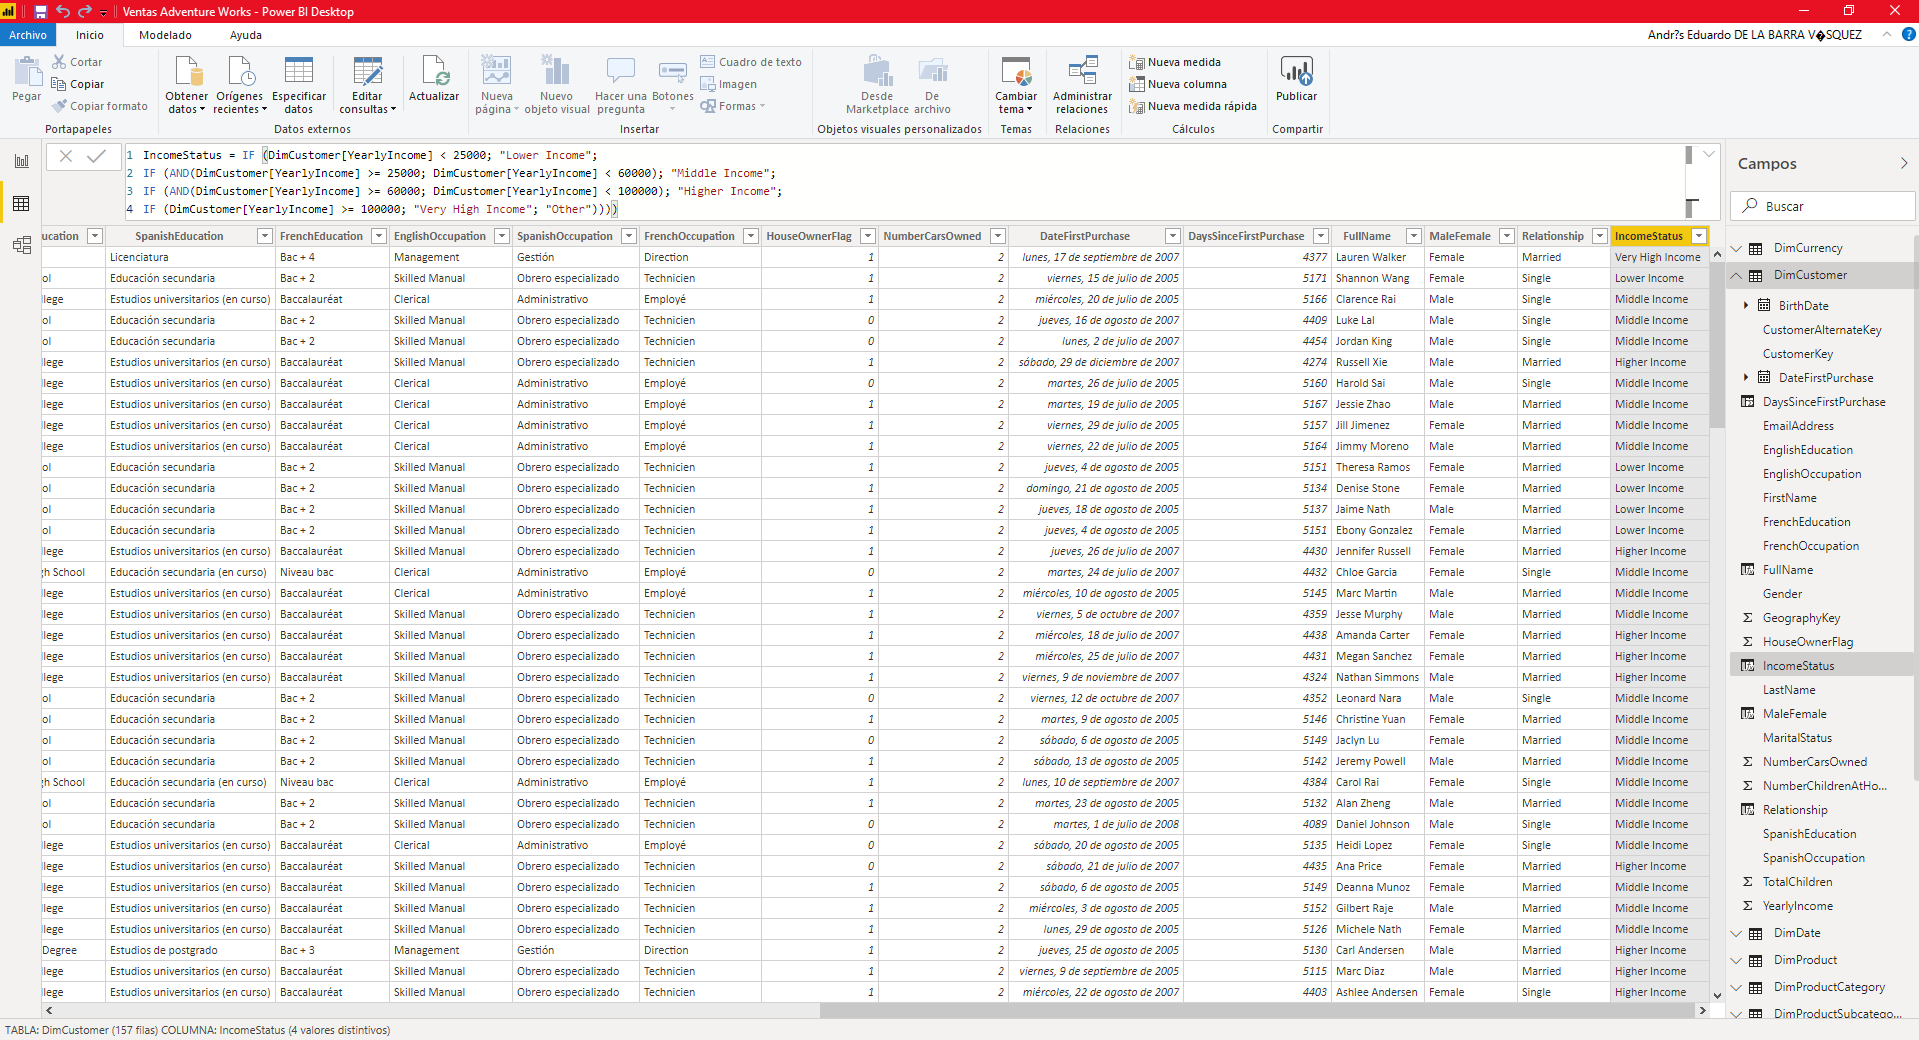
\includegraphics[width=18cm]{./Imagenes/imagen3}
		\end{center}
		\end{figure}
     
	\item 4. Ejercicio 2: Consulta de DimProductSubcategory
		\begin{figure}[H]
		\begin{center}
		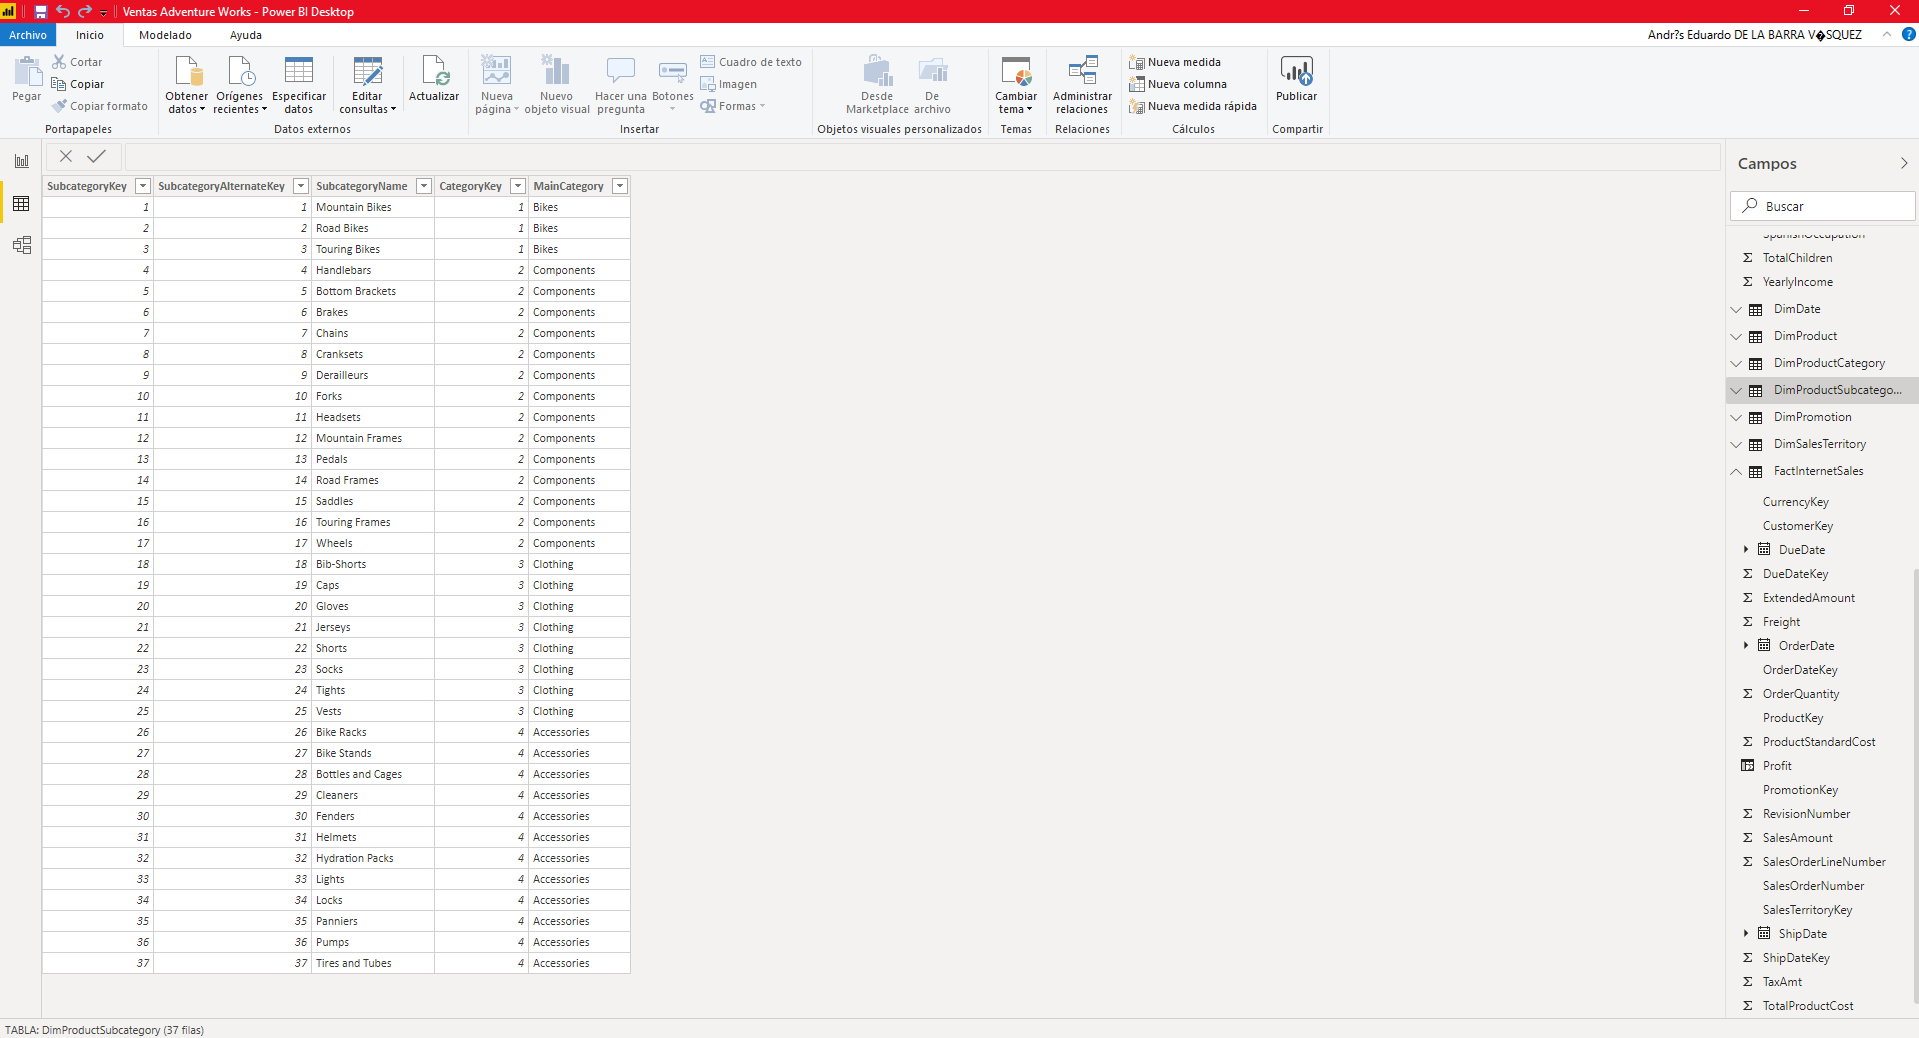
\includegraphics[width=18cm]{./Imagenes/imagen4}
		\end{center}
		\end{figure}
     
	\item 5. Ejercicio 2: Consulta DimPromotion
		\begin{figure}[H]
		\begin{center}
		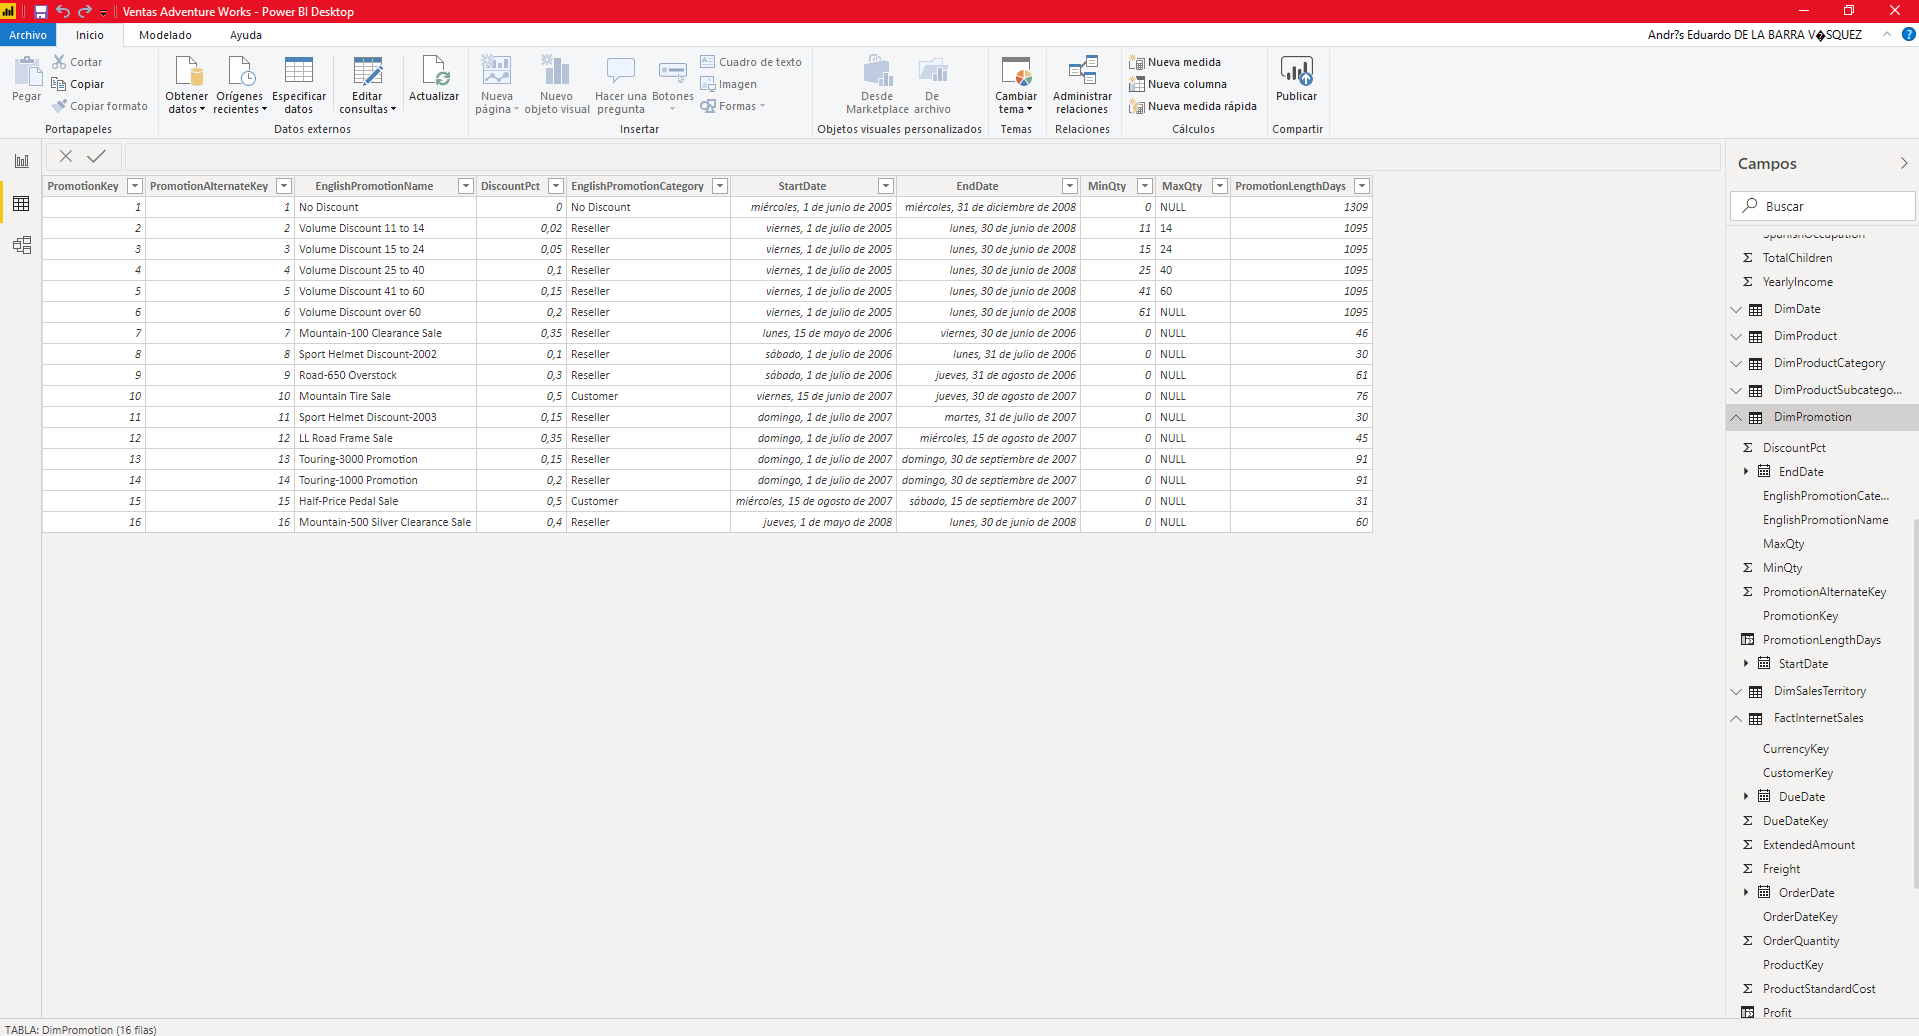
\includegraphics[width=18cm]{./Imagenes/imagen5}
		\end{center}
		\end{figure}
     
	\item 6. Ejercicio 2:Consulta FactInternetSales
		\begin{figure}[H]
		\begin{center}
		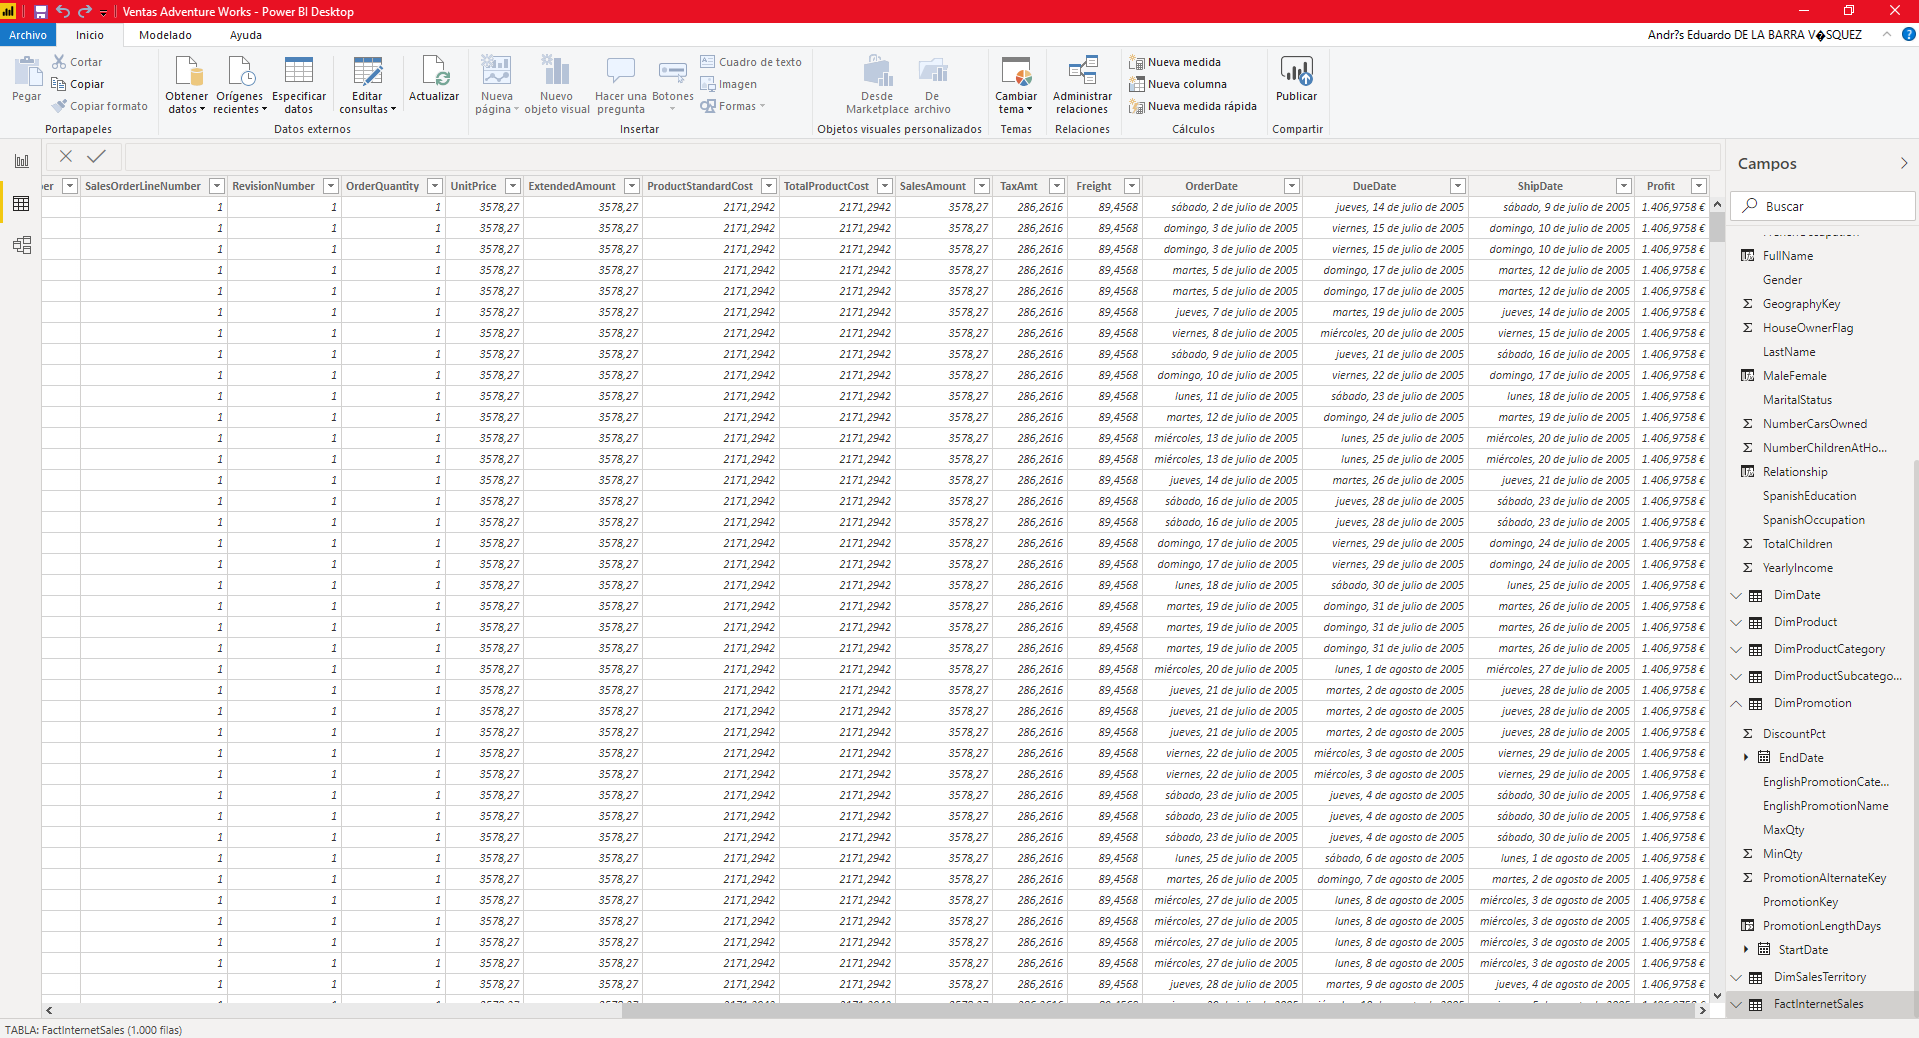
\includegraphics[width=18cm]{./Imagenes/imagen6}
		\end{center}
		\end{figure}
     




\end{itemize}
		


\end{document}
